\usetikzlibrary{matrix}
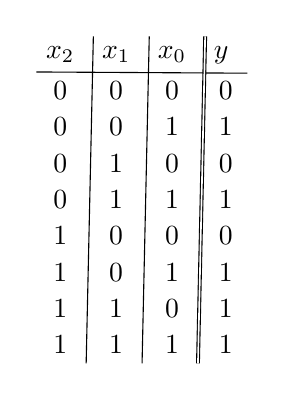
\begin{tikzpicture}
\matrix(dict)[matrix of nodes,%below=of game,
        nodes={align=center},
        %row 1/.style={anchor=south},
        %column 1/.style={nodes={text width=2cm,align=center}}
    ]{
        $x_2$ & $x_1$ & $x_0$ & $y$ \\
	 0 & 0 & 0 &  0\\
	 0 & 0 & 1 &  1\\
	 0 & 1 & 0 &  0\\
	 0 & 1 & 1 &  1\\
	 1 & 0 & 0 &  0\\
	 1 & 0 & 1 &  1\\
	 1 & 1 & 0 &  1\\
	 1 & 1 & 1 &  1\\
    };
    \draw(dict-1-1.south west)--(dict-1-4.south east);
    \draw(dict-1-1.north east)--(dict-9-1.south east);
    \draw(dict-1-2.north east)--(dict-9-2.south east);
    \draw[double](dict-1-3.north east)--(dict-9-3.south east);
\end{tikzpicture}